\documentclass{standalone}
\usepackage{tkz-euclide}
\usepackage{foekfont}
\usepackage[T1]{fontenc}
\begin{document}
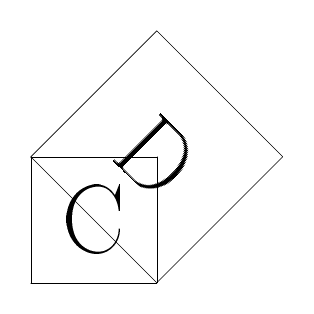
\begin{tikzpicture}[scale=0.4, label style/.style={font=\fontsize{128}{128}\selectfont}]
	\tkzInit [ymin=-0.1,ymax=8.1,xmin=-0.1,xmax=8.1] 
	\tkzClip
	\tkzDefPoint(0,0){a}
	\tkzDefPoint(4,0){b}
	\tkzDefPoint(4,4){c}
	\tkzDefPoint(0,4){d}
	\tkzDefPointBy[rotation= center d angle 90](b)
	\tkzGetPoint{e}
	\tkzDefPointBy[rotation= center b angle 270](d)
	\tkzGetPoint{f}
	\tkzDrawSegments(a,b b,c c,d d,a d,e)
	\tkzDrawSegments(b,f e,f d,b)
	\tkzDefMidPoint(d,b) \tkzGetPoint{m}
	\tkzLabelPoint(m){\fontencoding{T1}\fontfamily{foekfont}\fontsize{42}{42}\selectfont C}
	\tkzDefMidPoint(d,f) \tkzGetPoint{n}
	\tkzLabelPoint[rotate=-45](n){\fontencoding{T1}\fontfamily{foekfont}\fontsize{42}{42}\selectfont\MakeUppercase{D}}
	\end{tikzpicture}
\end{document}